\section{Design and Implementation}

At this point the project has a set of requirements to meet and basic solution approach has been outlined for each aspect of 
the project.
This section aims to inform the reader of the detailed design choices made and how this was implemented to achieve the final product.

\subsection{System model design}

\begin{figure}[ht]
    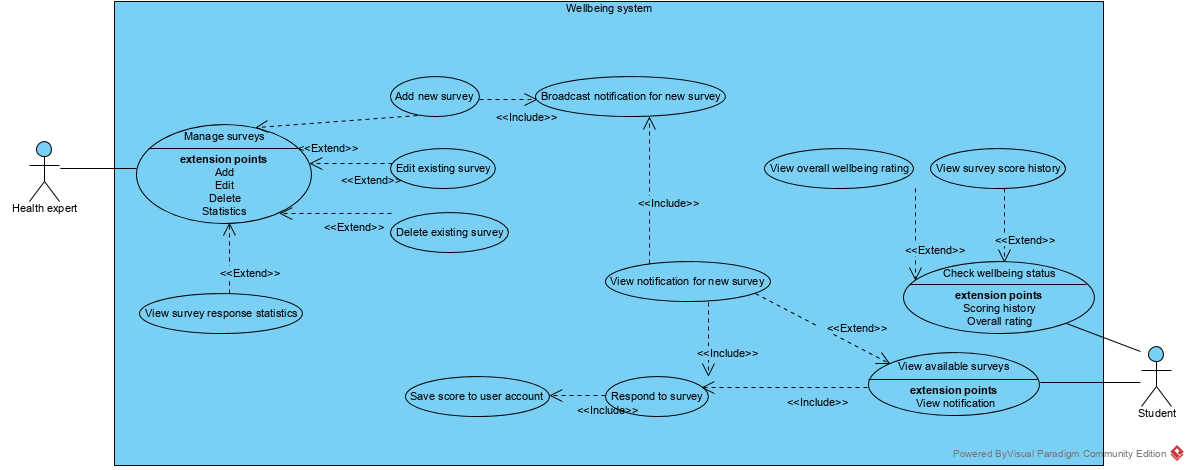
\includegraphics[width=450px]{images/system_model.png}
    \caption{Proposed system model}
\end{figure}


The proposed system model outlines the method in which an \textit{expert} can create, edit or delete a survey and how this can be 
fed to a student.
The main functionality to point out, that really links the two user types together, is how new survey send some sort notification 
to a (potentially) subscribed student; leading them to respond to the survey.
From the diagram, the reader should be able to see how a student will be able to either view surveys at their own will or be prompted
by a notification that had been sent out by some service.
The system outlines that there are really only two different categories of user that will use the system, this makes sense when looking
back at the articulation of the problem and the original brief given.

\subsection{Flow diagram}

An important process for the software solution is to be able to add and modify surveys for students to respond to.
The system model design does not go into much detail about this part of the system so it will be important to gain some clarity around this area.
Below is the proposed process flow diagram for what will occur when a user, of the system, attempts to add a new survey.
It outlines the need for authorisation (have permission to access such a resource) before carrying out two steps of validation of the
data provided.
If validation passes, then the survey and survey questions entries will be added to the database.
As mentioned in the system model design, there is a mention of the notification service that will alert students about a new survey they
can participate in.
The flow diagram shows how an expert can be prompted about sending out an alert to students, after submitting the survey.
That is where the system will then move onto executing the notification service, or just conclude the current process flow.

\begin{figure}[ht]
    \centering
    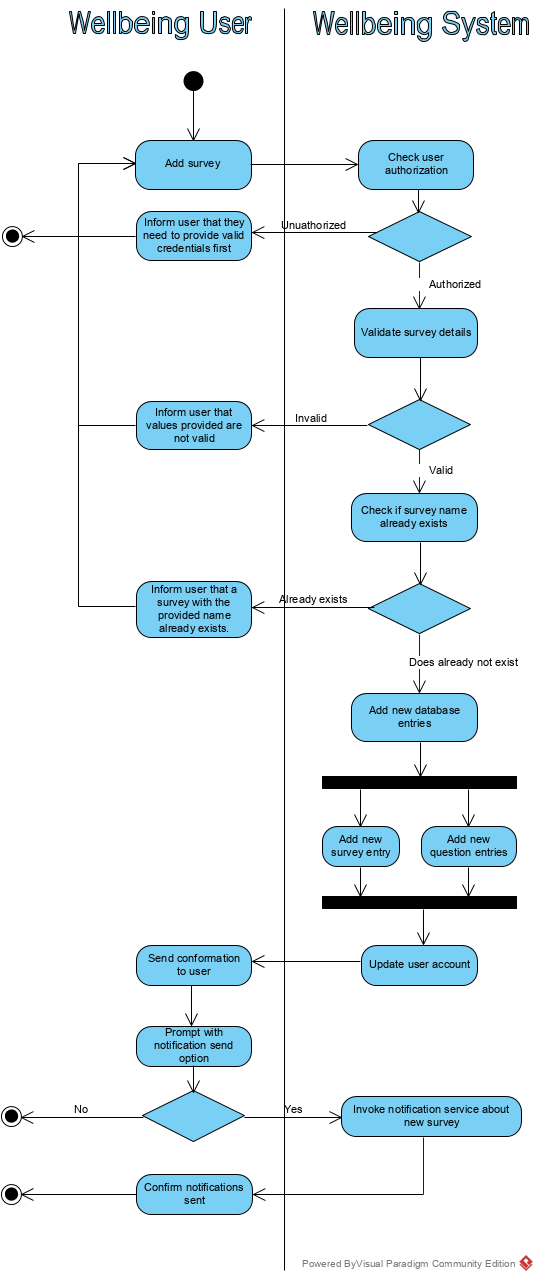
\includegraphics[width=150px]{images/flow_diagram.png}
    \caption{Flow diagram of the processes involved when an \textit{expert} adds a new survey}
\end{figure}

\clearpage

\subsection{REST API}
Talk about the REST api that you have developed in this section.
Give examples, maybe even give 

Maybe list out all the endpoints in a table or something.

\subsection{Database design}

Stuff to do with the database and the database schema.
You can use your JDL thing to represent it here if you really wan to.

\subsubsection{Java Persistence API}
\begin{enumerate}
    \item How entities are defined in the java code 
    \item Talk about JDBC or something as in the way you connected to the database from java
    \item Include the configuration stuff you've also done and explain what it does.
    \item Talk about Repository files and how they act as the interface between the java app and the database
    \item Talk about derrived methods for the repositories
\end{enumerate}


\subsection{Spring security}

Talk about spring security aspects that you have implemented
oauth2 and jwt are good examples
what else?



\subsection{REACT client}
Talk about everything to do with the implementation of the REST client
State how you started off from that OKTA example and worked from there. 
